\documentclass{article}
\usepackage[top=25truemm,bottom=20truemm,left=20truemm,right=20truemm]{geometry}

\usepackage{amsmath}
\usepackage{amssymb}
\usepackage{amsfonts}
\usepackage{mathrsfs}
\usepackage{latexsym}
\usepackage{bm}
\usepackage[dvipdfmx]{graphicx}
\usepackage{physics}
\usepackage{braket}
\usepackage{float}

\usepackage{comment}

\title{Notes on density functional theory}
\author{Ryota Masuki}
\date{\today}

\begin{document}
\maketitle

\section{Pseudopotential methods}
\subsection{Norm-conserving Pseudopotential}
The idea of the norm-conserving pseudopotential was conceived by Hamman, et al~\cite{PhysRevLett.43.1494}.
The important point is that the preservation of the derivative of the phase shift follows from the norm-conserving condition,
which theoretically supports the transferability of this pseudopotential.

We first explain the Norm-conserving pseudopotential in a one-body problem.
How to combine the idea with DFT is explained later.

The norm-conserving pseudopotential is the angular-momentum-dependent pseudopotential with the form
\begin{align}
  V^{\text{ps}} = \sum_{L:(lm)} \ket{lm} V^{\text{ps}}_l(r) \bra{lm}
\end{align}
that satisfy the following condition.
\begin{enumerate}
  \item The pseudo (radial) wavefunction $R^{\text{ps}}_l(r)$ satisfy the Schroedinger equation
  \begin{align}
    \Bigl[
      - \frac{\hbar^2}{2m} \frac{d^2}{dr^2} + \frac{l(l+1)\hbar^2}{2mr^2} + V^{\text{ps}}_l(r)
    \Bigr] rR^{\text{ps}}_l(r) = E_l r R^{\text{ps}}_l(r).
  \end{align}
  Note that the all-electron radial wavefunction $R^{\text{ae}}_l(r)$ satisfies
  \begin{align}
    \Bigl[
      - \frac{\hbar^2}{2m} \frac{d^2}{dr^2} + \frac{l(l+1)\hbar^2}{2mr^2} + V(r)
    \Bigr] rR^{\text{ps}}_l(r) = E_l r R^{\text{ps}}_l(r),
  \end{align}
  where $V(r)$ is the original one-body potential which is independent of angular momentum $lm$.
  \item The pseudowavefunctions $R^{\text{ps}}_l(r)$ don't have zero-points inside the core region $r<r_c$ and satisfy the norm-conserving condition
  \begin{align}
    \int_0^{r_c} dr r^2 (R^{\text{ps}}_l(r))^2 = \int_0^{r_c} dr r^2 R_l^2(r)
  \end{align}
  We can prove that the derivative of the phase shift with respect to the energy at $E = E_l$ is preserved if the norm-conserving condition is satisfied~\cite{PhysRevLett.43.1494, Fujiwara_Kotaidenshikouzou}, which I abbreviate the proof here.
  \item The pseudowavefunctions exactly match the original wavefunction outside the core region.
  \begin{align}
   R^{\text{ps}}_l(r)= R_l(r) \text{\ }(r > r_c)
  \end{align}
\end{enumerate}

\subsubsection{Generation of norm-conserving pseudopotentials}
The generation of norm-conserving pseudopotentials are done as follows.
\begin{enumerate}
  \item Calculate the original wavefunction $R_l(r)$.\\
  We start with solving the exact one-body problem for atoms. In case of DFT, we solve the all-electron DFT for atoms.
  \item Determine the pseudowavefunction $R^{\text{ps}}_l(r)$ that safisfy the conditions discussed above.\\
  In principle, the choice of $R^{\text{ps}}_l(r)$ is arbitrary, as long as it satisfies the norm-conserving condition, etc.
  However, it is better to choose ones that are more smooth and transferable (I'm not familiar with how to make pseudopotentials with high transferability, though).
  \item Calculate pseudopotential
  \begin{align}
    V^{\text{ps}}_l(r) = E_l - \frac{l(l+1)\hbar^2}{2mr^2} + \frac{1}{rR^{\text{ps}}_l(r)}  \frac{\hbar^2}{2m} \frac{d^2}{dr^2} [rR^{\text{ps}}_l(r)]
  \end{align}
\end{enumerate}
\subsubsection{Combination of norm-conserving potentials with DFT}
The Kohn-Sham equation solved in all-electron DFT for atoms is 
\begin{align}
  \Bigl[
    - \frac{\hbar^2}{2m} \frac{d^2}{dr^2} + \frac{l(l+1)\hbar^2}{2mr^2} +  v_{\text{ext}}(r) + v_H(r;n) + v_{xc}(r;n)
  \Bigr] rR_l(r) = E_l r R_l(r).
\end{align}
On the other hand, the Kohn-Sham equation with the pseudopotential will look like
\begin{align}
  \Bigl[
    - \frac{\hbar^2}{2m} \frac{d^2}{dr^2} + \frac{l(l+1)\hbar^2}{2mr^2} +  v^{\text{ps:ion}}_l(r) + v_H(r;n^{\text{ps}}) + v_{xc}(r;n^{\text{ps}} + n_c)
  \Bigr] rR^{\text{ps}}_l(r) = E_l r R^{\text{ps}}_l(r).
\end{align}
where
\begin{align}
  n(\bm{r}) = \sum_{i: \text{occupied valence and core}} |\psi_i (\bm{r}) |^2
\end{align}
is the all-electron density and 
\begin{align}
  n^{\text{ps}}(\bm{r}) = \sum_{v: \text{occupied valence}} |\psi_v^{\text{ps}} (\bm{r}) |^2
\end{align}
is the density calculated from the pseudo density.
$n_c$ is the density of the core electron density, which is fixed in the frozen core approximation (?).
Thus, the ionic pseudopotential is calculated as 
\begin{align}
  V^{\text{ps:ion}} = \sum_{lm} \ket{lm} v^{\text{ps:ion}}_l(r)  \bra{lm},
\end{align}
\footnote{In textbooks, we see the form
\begin{align}
  V^{\text{ps:ion}} = V_{\text{local}}(r) + \sum_{lm} \ket{lm} v^{\text{ps:ion}}_l(r)  \bra{lm},
\end{align}
where $V_{\text{local}}(r) $ is the $l$-independent term.
Here, the definition of $V_{\text{local}}(r)$ is arbitrary because it can be included in $v^{\text{ps:ion}}_l$.
I suppose that  $V_{\text{local}}(r)$ is chosen by numerical reasons considering that we can use only finite numbers of $lm$'s in numerical calculations (Need confirmation).
}
where 
\begin{align}
  v^{\text{ps:ion}}_{l}(r) = V^{\text{ps}}_l(r) - v_H(r;n^{\text{ps}}) - v_{xc}(r;n).
\end{align}

\subsubsection{Approximations in norm-conserving pseudopotentials}
Norm-conserving pseudopotentials are exact
\begin{itemize} 
  \item for the wavefunction outside the core region and the total charge inside the core region
  \item for the same quantum number $n$ as the eigen state $R_{nl}$ used for the generation of the pseudopotential (Note that we have abbreviated the primary quantum number $n$ so far!)
  \item when the charge density and the potential exactly matches the original atomic problem.
\end{itemize}
They are not exact when any of the above conditions is not satisfied. The third condition is satisfied only when we solve the same atomic problem as the generation of the pseudopotential.

\subsection{Ultrafast pseudopotential}
The ultrasoft pseudopotential was conceived by D. Vanderbilt~\cite{PhysRevB.41.7892}.
The most prominent feature of the ultrasoft pseudopotentials is that the transferability can be systematically improved by increasing the number of reference energies.

\subsubsection{The case of one-state}
We consider a one-body spherically symmetric problem.
\begin{align}
  \Bigl(
    \frac{-\hbar^2}{2m} \frac{d^2}{dr^2}
    + V(r)
    + \frac{l(l+1)\hbar^2}{2mr^2} 
  \Bigr)r R_{nl}(r)
  = 
  \epsilon_{nl} r R_{nl}(r),
\end{align}
where the radial wavefunction $R_{nl}(r)$ is defined as 
\begin{align}
  \psi_{nlm}(\bm{r}) = R_{nl}(r) Y_{lm}(\hat{\bm{r}}),
\end{align}
using the full wavefunction $\psi_{nlm}(\bm{r})$.
Here, we consider a pseudo wavefunction 
\begin{align}
  \phi_{nlm}(\bm{r}) = R^{\text{ps}}_{nl}(r) Y_{lm}(\hat{\bm{r}}),
\end{align}
which 
\begin{itemize}
  \item smoothly connects to $\psi_{nl}$ at $r = r_c$.
  \item satisfies the norm-conserving condition
  \begin{align}
    \int_0^{R} r^2 R_{nl}^2 (r) = \int_0^{R} r^2 ( R^{\text{ps}}_{nl} (r) )^2\text{\ \ }(R > r_c)
  \end{align}
\end{itemize}
Here, we define 
\begin{align}
  \ket{\chi_{nlm}} 
  &= \Bigl(\epsilon_{nl} + \frac{\hbar^2\nabla^2}{2m} - V \Bigr)\ket{\phi_{nlm}}
  \nonumber
  \\&=
  Y_{lm}(\hat{\bm{r}})
  \frac{1}{r}
  \times
  \Bigl(\epsilon_{nl} + \frac{\hbar^2}{2m} \frac{d^2}{dr^2} - \frac{l(l+1)\hbar^2}{2mr^2} - V \Bigr) r R^{\text{ps}}_{nl}(r)
  \nonumber
  \\&= 
  R^{\chi}_{nl}(r) Y_{lm}(\hat{\bm{r}})
\end{align}
\begin{align}
  V_{NL} 
  &= \sum_{lm} \frac{\ket{\chi_{nlm}}_R\bra{\chi_{nlm}}_R}{\braket{\chi_{nl} | \phi_{nl}}_R}
  \nonumber
  \\&=
  \sum_{l} \hat{P_l} \frac{\ket{\chi_{nl}}_R\bra{\chi_{nl}}_R}{\braket{\chi_{nl} | \phi_{nl}}_R} \hat{P_l},
\end{align}
Note that 
\begin{align}
  \braket{\chi_{nl} | \phi_{nl}}_R
  &= \braket{\chi_{nlm} | \phi_{nlm}}_R
  \nonumber
  \\&=
  \int_0^R dr r 
  (R^{\text{ps}}_{nl}(r))^* 
  \Bigl(
    \epsilon_{nl} 
    + \frac{\hbar^2}{2m}\frac{d^2}{dr^2} 
    - \frac{l(l+1)\hbar^2}{2mr^2} - V(r) \
  \Bigr) r R^{\text{ps}}_{nl}(r)
  \nonumber
  \\&=
  \int_0^R dr r^2 (R^{\chi}_{nl}(r) )^* R^{\text{ps}}_{nl}(r)
\end{align}
is independent of the magnetic quantum number $m$.
For arbitrary state $\widetilde{\psi}_{lm}(\bm{r}) = \widetilde{R}(r) Y_{lm}(\hat{\bm{r}})$ with angular momentum $lm$, $\ket{\chi_{nlm}}_R\bra{\chi_{nlm}}_R$ operates as
\begin{align}
  \ket{\chi_{nlm}}_R\bra{\chi_{nlm}}_R \widetilde{\psi}_{lm}(\bm{r}) 
  = 
  \chi_{lm}({\bm{r}}) \times \int_0^R dr r^2 (R^{\text{ps}}_{nl}(r))^* \widetilde{R}(r).
\end{align}
\begin{comment}
where
\begin{align}
  r R^{\chi}(\bm{r}) = 
  \Bigl(
    \epsilon_{nl} 
    + \frac{\hbar^2}{2m}\frac{d^2}{dr^2} 
    - \frac{l(l+1)\hbar^2}{2mr^2} - V(r) \
  \Bigr) r R^{\text{ps}}_{nl}(r)
\end{align}
\end{comment}
$V_{NL}$ satisfies
\begin{align}
 \Bigl( - \frac{\hbar^2\nabla^2}{2m} + V(\bm{r}) + V_{NL}\Bigr) \phi_{nlm}(\bm{r}) = \epsilon_{nl} \phi_{nlm}(\bm{r}).
\end{align}

\subsubsection{Extension to multiple states}
We next consider multiple $n$ for each $l$.
We again consider a one-body spherically symmetric problem.
\begin{align}
  \Bigl(
    \frac{-\hbar^2}{2m} \frac{d^2}{d2r^2}
    + V(r)
    + \frac{l(l+1)\hbar^2}{2mr^2} 
  \Bigr)r R_{nl}(r)
  = 
  \epsilon_{nl} r R_{nl}(r),
\end{align}
where the radial wavefunction $R_{nl}(r)$ is defined as 
\begin{align}
  \psi_{nlm}(\bm{r}) = R_{nl}(r) Y_{lm}(\hat{\bm{r}}),
\end{align}
using the full wavefunction $\psi_{nlm}(\bm{r})$.
Here, we consider a pseudo wavefunction 
\begin{align}
  \phi_{nlm}(\bm{r}) = R^{\text{ps}}_{nl}(r) Y_{lm}(\hat{\bm{r}}),
\end{align}
which 
\begin{itemize}
  \item smoothly connects to $\psi_{nl}$ at $r = r_c$.
  \item does NOT NECESSARILY satisfy the norm-conserving condition
\end{itemize}
Following the procedure in the one-state case, we define
\begin{align}
  \ket{\chi_{nlm}} 
  &= \Bigl(\epsilon_{nl} + \frac{\hbar^2\nabla^2}{2m} - V \Bigr)\ket{\phi_{nlm}}
  \nonumber
  \\&=
  Y_{lm}(\hat{\bm{r}})
  \frac{1}{r}
  \times
  \Bigl(\epsilon_{nl} + \frac{\hbar^2}{2m} \frac{d^2}{dr^2} - \frac{l(l+1)\hbar^2}{2mr^2} - V \Bigr) r R^{\text{ps}}_{nl}(r)
  \nonumber
  \\&= 
  R^{\chi}_{nl}(r) Y_{lm}(\hat{\bm{r}}).
\end{align}
Here, we define 
\begin{align}
  Q_{lij} 
  &= 
  \braket{\psi_{ilm} | \psi_{jlm}}_R - \braket{\phi_{ilm} | \phi_{jlm}}_R 
  \nonumber
  \\&=
  \int_0^R dr r^2 [ R_{il}^*(r) R_{jl}(r) - (R^{\text{ps}}_{il}(r))^* R^{\text{ps}}_{jl}(r) ],
\end{align}
\begin{align}
  B_{lij} 
  &= 
   \braket{\phi_{ilm} | \epsilon_{jl} + \frac{\hbar^2\nabla^2}{2m} - V|\phi_{jlm}}_R 
  \nonumber
  \\&=
  \braket{\phi_{ilm} | \chi_{jlm}}_R 
  \nonumber
  \\&=
  \int_0^R dr 
  r(R^{\text{ps}}_{il}(r))^* 
  \Bigl(
    \epsilon_{jl} + \frac{\hbar^2}{2m} \frac{d^2}{dr^2} - \frac{l(l+1)\hbar^2}{2mr^2} - V(r)
  \Bigr)
  r R^{\text{ps}}_{jl}(r).
\end{align}
Both $Q_{lij}$ and $B_{lij}$ are independent of the magnetic quantum number $m$, although $m$ appears when we define them with braket formalism.
$Q_{lij}$ is the correction of the charge in the core region that we need to add to the pseudo density in order to obtain the correct total charge.
$B_{lij}$ satisfies $B_{lij} - B_{lji}^* = (\epsilon_{il} - \epsilon_{jl}) Q_{lij}$, which can be shown as
\begin{align}
  B_{lij} - B_{lji}^* 
  &=
  (\epsilon_{jl} - \epsilon_{il}) \int_0^R dr r^2 (R^{\text{ps}}_{il}(r))^* R^{\text{ps}}_{jl}(r)
  + \frac{\hbar^2}{2m} \int_0^R r (R^{\text{ps}}_{il}(r))^* \frac{d^2}{dr^2} rR^{\text{ps}}_{jl}(r) - rR^{\text{ps}}_{jl}(r) \frac{d^2}{dr^2} (rR^{\text{ps}}_{il}(r))^* 
  \nonumber
  \\&=
  (\epsilon_{jl} - \epsilon_{il}) \int_0^R dr r^2 (R^{\text{ps}}_{il}(r))^* R^{\text{ps}}_{jl}(r)
  + \frac{\hbar^2}{2m}
  \Bigl[
    (R^{\text{ps}}_{il}(r))^* \frac{d}{dr} rR^{\text{ps}}_{jl}(r) - rR^{\text{ps}}_{jl}(r) \frac{d}{dr} (rR^{\text{ps}}_{il}(r))^* 
  \Bigr]_0^R
  \nonumber
  \\&=
  (\epsilon_{jl} - \epsilon_{il}) \int_0^R dr r^2 (R^{\text{ps}}_{il}(r))^* R^{\text{ps}}_{jl}(r)
  + \frac{\hbar^2}{2m}
  \Bigl[
    (R_{il}(r))^* \frac{d}{dr} rR_{jl}(r) - rR_{jl}(r) \frac{d}{dr} (rR_{il}(r))^* 
  \Bigr]_0^R
  \nonumber
  \\&=
  (\epsilon_{jl} - \epsilon_{il}) \int_0^R dr r^2 (R^{\text{ps}}_{il}(r))^* R^{\text{ps}}_{jl}(r)
  + \frac{\hbar^2}{2m} \int_0^R r (R_{il}(r))^* \frac{d^2}{dr^2} rR_{jl}(r) - rR_{jl}(r) \frac{d^2}{dr^2} (rR_{il}(r))^* 
  \nonumber
  \\&=
  (\epsilon_{jl} - \epsilon_{il}) \int_0^R dr r^2 (R^{\text{ps}}_{il}(r))^* R^{\text{ps}}_{jl}(r) - (\epsilon_{jl} - \epsilon_{il}) \int_0^R dr r^2 (R_{il}(r))^* R_{jl}(r)
  \nonumber 
  \\&= (\epsilon_{il} - \epsilon_{jl}) Q_{lij}
\end{align}
We used that $R_{il} = R^{\text{ps}}_{jl}$ at $r > r_c$ (from the second to third line) and that $R_{il}Y_{lm}$ is the eigenstate of $ - \frac{\hbar^2\nabla^2}{2m} + V(\bm{r}) $ (from the fourth to the fifth line). Note that a similar transformation as that from the fourth to the fifth line cannot be used for $R^{\text{ps}}_{il}$ because it is not an eigenstate of the considering operator.
We also define
\begin{align}
  \ket{\beta_{ilm}} = \sum_j (B^{-1}_l)_{ji} \ket{\chi_{jlm}},
\end{align}
which satisfy
\begin{align}
  \braket{\phi_{ilm} | \beta_{jl'm'}} = \delta_{ll'} \delta_{mm'} \delta_{ij}
\end{align}
Here, IF $Q_{lij} = 0$ (norm-conserving condition is SATISFIED), we can construct an Hermitian operator
\begin{align}
  V_{NL} 
  &= 
  \sum_{lm,ij} B_{lij} \ket{\beta_{ilm}} \bra{\beta_{jlm}}
  \nonumber
  \\&=
  \sum_{lm,ij} (B_{l}^{-1})_{ij}^* \ket{\chi_{ilm}} \bra{\chi_{jlm}},
\end{align}
which satisfies
\begin{align}
  \Bigl(
    - \frac{\hbar^2\nabla^2}{2m} + V(\bm{r}) + V_{NL}
  \Bigr)
  \ket{\psi_{nlm}} = \epsilon_{nl}\ket{\psi_{nlm}}
\end{align}
as in the one-state case.

Let's now relax the norm-conserving condition.
We define 
\begin{align}
  S = 1 + \sum_{lijm} Q_{lij} \ket{\beta_{ilm}} \bra{\beta_{jlm}}
\end{align}
Then, we get
\begin{align}
  \braket{\phi_{ilm} | S | \phi_{jl'm'}}_R = \braket{\psi_{ilm} | \psi_{jl'm'}}
\end{align}
Now, we try to minimize the energy functional 
\begin{align}
a
\end{align}


\subsection{Projector Augmented Wave (PAW) method}
\subsubsection{Theory}
The all electron wavefunction $\ket{\Psi}$ is written by 
\begin{align}
\ket{\Psi} = \mathcal{T} \ket{\widetilde{\Psi}}
\end{align}
using the pseudo wavefunction $\ket{\widetilde{\Psi}}$. Here, the PAW transformation, which transforms the PS wavefunction to AE wavefunction, is 
\begin{align}
  \mathcal{T} = 1 + \sum_{\bm{R}\alpha} \mathcal{T}_{\bm{R}\alpha},
\end{align}
where $\mathcal{T}_{\bm{R}\alpha}$ operates in a sphere surrounding the atom $\bm{R}\alpha$.

Here, for a set of complete set in the sphere $\ket{\widetilde{\phi}_{\bm{R}\alpha, nL}}$, we assume that 
\begin{align}
  \ket{{\phi}_{\bm{R}\alpha, nL}} = (1 + \mathcal{T}_{\bm{R}\alpha}) \ket{\widetilde{\phi}_{\bm{R}\alpha, nL}}.
\end{align}
Then, using the projecor functions $\ket{\widetilde{p}_{\bm{R}\alpha,nL}}$, which satisfies
\begin{align} 
  \sum_{nL} \ket{\widetilde{\phi}_{\bm{R}\alpha, nL}} \bra{\widetilde{p}_{\bm{R}\alpha, nL}} = 1
\end{align}
for all atoms $\bm{R}\alpha$, the PAW transformation can be explicitly written as 
\begin{align}
  \mathcal{T} = 1 + \sum_{i = (\bm{R}\alpha, nL)} (\ket{\phi_i} - \ket{\widetilde{\phi}_i}) \bra{\widetilde{p}_i}.
\end{align}

\subsubsection{Operators}
For any one-body operator $A$, 
\begin{align}
  \widetilde{A} 
  &= \mathcal{T}^\dag A \mathcal{T}
  \\&=
  A + 
  \sum_{i = (\bm{R}_1\alpha_1,n_1L_1),j = (\bm{R}_2\alpha_2, n_2 L_2)}
  \ket{\widetilde{p}_i}
  (\braket{\phi_i | A | \phi_j} - 
  \braket{\widetilde{\phi}_i | A | \widetilde{\phi}_j})
  \bra{\widetilde{p}_j}
  + \Delta A
\end{align}
Please see Ref.~\cite{PhysRevB.50.17953} for details of $\Delta A$.
When $A$ is a semilocal operator, $\Delta A$ vanishes, and the second term can be rewritten as 
\begin{align}
  \widetilde{A} 
  &= \mathcal{T}^\dag A \mathcal{T}
  \\&=
  A + 
  \sum_{\bm{R}\alpha,n_1L_1, n_2 L_2}
  \ket{\widetilde{p}_{\bm{R}\alpha,n_1L_1}}
  (\braket{\phi_{\bm{R}\alpha,n_1L_1} | A | \phi_{\bm{R}\alpha,n_2L_2}} - 
  \braket{\widetilde{\phi}_{\bm{R}\alpha,n_1L_1} | A | \widetilde{\phi}_{\bm{R}\alpha,n_2L_2}})
  \bra{\widetilde{p}_{\bm{R}\alpha,n_2L_2}}
\end{align}
The charge density is given by
\begin{align}
  n(\bm{r}) = \widetilde{n}(\bm{r}) + n^1(\bm{r}) - \widetilde{n}^1(\bm{r}),
\end{align}
where
\begin{align}
\widetilde{n}(\bm{r}) =  \sum_{n\bm{k}} f_{n\bm{k}} |\widetilde{\psi}_{n\bm{k}}(\bm{r})|^2 
\end{align}
\begin{align}
  {n}^1(\bm{r}) =  \sum_{n\bm{k}} \sum_{\bm{R}\alpha, nL, n'L'} f_{n\bm{k}} 
  \braket{\widetilde{\psi}_{n\bm{k}} | \widetilde{p}_{\bm{R}\alpha, nL}} 
  \phi^*_{\bm{R}\alpha, nL}(\bm{r})
  \phi^*_{\bm{R}\alpha, n'L'}(\bm{r})
  \braket{ \widetilde{p}_{\bm{R}\alpha, n'L'} | \widetilde{\psi}_{n\bm{k}} } 
\end{align}
\begin{align}
  \widetilde{n}^1(\bm{r}) =  \sum_{n\bm{k}} \sum_{\bm{R}\alpha, nL, n'L'} f_{n\bm{k}} 
  \braket{\widetilde{\psi}_{n\bm{k}} | \widetilde{p}_{\bm{R}\alpha, nL}} 
  \widetilde{\phi}^*_{\bm{R}\alpha, nL}(\bm{r})
  \widetilde{\phi}^*_{\bm{R}\alpha, n'L'}(\bm{r})
  \braket{ \widetilde{p}_{\bm{R}\alpha, n'L'} | \widetilde{\psi}_{n\bm{k}} } 
\end{align}

\begin{figure}[H]
  \begin{center}
  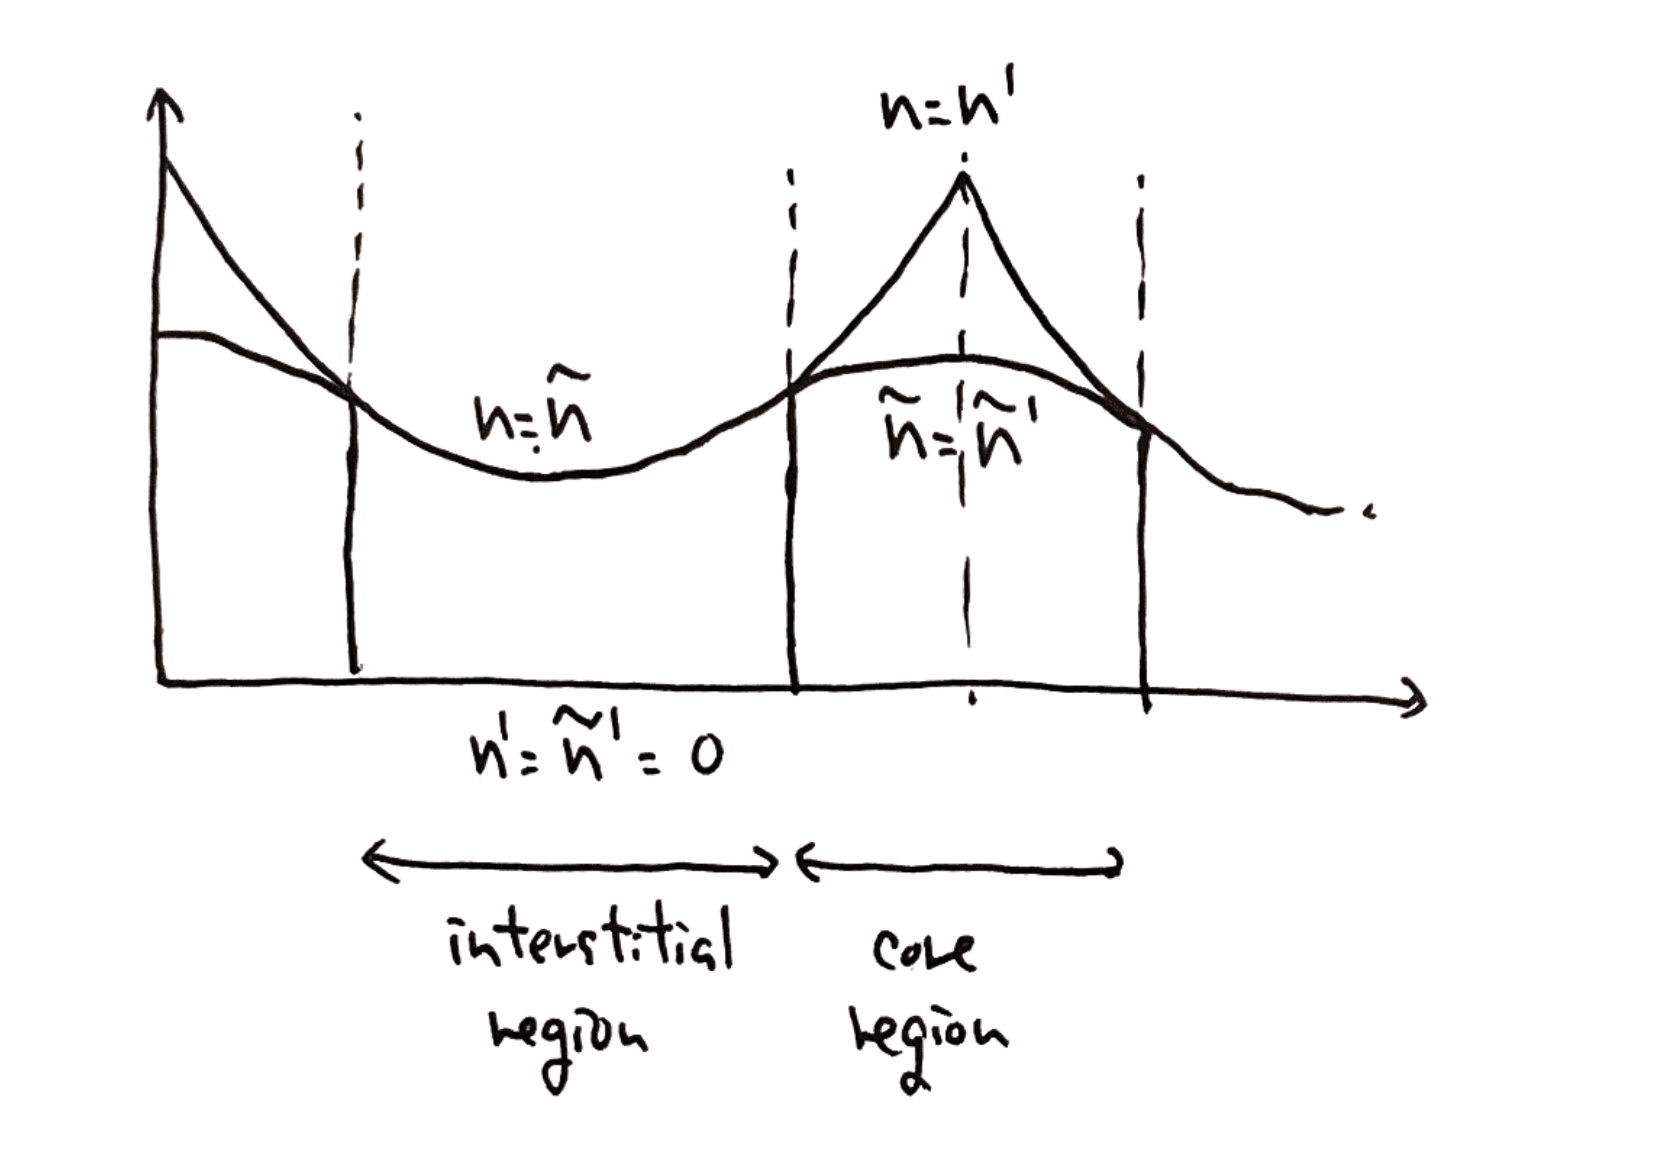
\includegraphics[width=100mm]{figures/PAW_charge.png}
  \caption{Schematic of the PAW charge densities.}
  \end{center}
\end{figure}

\subsubsection{Total energy}
Under LDA, the total energy functional is 
\begin{align}
  E &=
  \sum_{n\bm{k}} f_{n\bm{k}} \braket{\phi_{n\bm{k}} | \frac{-\hbar^2\nabla^2}{2m} | \phi_{n\bm{k}}}
  \nonumber
  \\&+
  \frac{e^2}{2} \int d\bm{r}d\bm{r}' \frac{(n(\bm{r})+ n^Z(\bm{r})) (n(\bm{r}')+ n^Z(\bm{r}'))}{|\bm{r} - \bm{r}'|}
  + \int d\bm{r} n(\bm{r})\epsilon_{xc}(n(\bm{r})),
\end{align}
where $n^Z$ is the (charge) density of nuclei in the unit of $-e$.
With a cumbersome calculation, we can prove that $E = \widetilde{E} + E^1 - \widetilde{E}^1$ with
\begin{align} 
  \widetilde{E} &= 
  \sum_{n\bm{k}} f_{n\bm{k}} \braket{\widetilde{\psi}_{n\bm{k}} | \frac{-\hbar^2\nabla^2}{2m} |\widetilde{\psi}_{n\bm{k}} }
  + \frac{e^2}{2}\int d\bm{r}d\bm{r}' \frac{(\widetilde{n} + \hat{n})(\widetilde{n} + \hat{n})}{|\bm{r}-\bm{r}'|}
  \nonumber \\&
  + \int d\bm{r} \widetilde{n}(\bm{r})\bar{v}(\bm{r})
  + \int d\bm{r} \widetilde{n}(\bm{r})\epsilon_{xc}(\widetilde{n}(\bm{r})),
  \label{eq:tildeE}
\end{align}
\begin{align} 
  {E}^1 &= 
  \sum_{n\bm{k}} \sum_{\bm{R}\alpha, nL, n'L'}f_{n\bm{k}} 
  \braket{\widetilde{\psi}_{n\bm{k}} | \widetilde{p}_{\bm{R}\alpha, nL}}
  \braket{\phi_{\bm{R}\alpha, nL}| \frac{-\hbar^2\nabla^2}{2m} |\phi_{\bm{R}\alpha, n'L'}}
  \braket{\widetilde{p}_{\bm{R}\alpha, n'L'}|\widetilde{\psi}_{n\bm{k}} }
  \nonumber\\&
  + \frac{e^2}{2}\int d\bm{r}d\bm{r}' \frac{({n}^1 + n^Z)({n}^1 + n^Z)}{|\bm{r}-\bm{r}'|}
  + \int d\bm{r} {n}^1(\bm{r})\epsilon_{xc}({n}^1(\bm{r})),
\end{align}
\begin{align} 
  \widetilde{E}^1 &= 
  \sum_{n\bm{k}} \sum_{\bm{R}\alpha, nL, n'L'}f_{n\bm{k}} 
  \braket{\widetilde{\psi}_{n\bm{k}} | \widetilde{p}_{\bm{R}\alpha, nL}}
  \braket{\widetilde{\phi}_{\bm{R}\alpha, nL}| \frac{-\hbar^2\nabla^2}{2m} |\widetilde{\phi}_{\bm{R}\alpha, n'L'}}
  \braket{\widetilde{p}_{\bm{R}\alpha, n'L'}|\widetilde{\psi}_{n\bm{k}} }
  \nonumber\\&
  + \frac{e^2}{2}\int d\bm{r}d\bm{r}' \frac{(\widetilde{n}^1 + \hat{n})(\widetilde{n}^1 + \hat{n})}{|\bm{r}-\bm{r}'|}
  + \int d\bm{r} \widetilde{n}^1(\bm{r})\bar{v}(\bm{r})
  + \int d\bm{r} \widetilde{n}^1(\bm{r})\epsilon_{xc}(\widetilde{n}^1(\bm{r})).
\end{align}
Note that 
\begin{itemize}
  \item $\bar{v}$ is arbitrary potential which vanishes in the interstitial region.
  \item $\hat{n}$ is the compensation charge density that cannot be distinguished from $n + n^Z - \widetilde{n} = n^1 + n^Z - \widetilde{n}^1$ when seen from the interstitial region. $\widetilde{n} + \hat{n}$ is a smooth charge density with charge neutrality. ${n}^1 + n^Z$ in $E^1$ and $\ widetilde{n}^1 + \hat{n}$ in $\widetilde{E}^1$ are confined in the core region. These densities have the same charge as the charge in the core region. These Coulomb integrals in $E^1$ and $\widetilde{E}^1$ are infinite, but the divergent term cancel with each other.
\end{itemize}
The compenastion charge  desnity $\hat{n}$ is determined as
\begin{align}
  \hat{n}_{\bm{R}\alpha} = \sum_L g_{\bm{R}\alpha L}(\bm{r}) Q_{\bm{R}\alpha L},
\end{align}
\begin{align}
  g_{\bm{R}\alpha L} = 
  C_{\alpha l} |\bm{r} - \bm{R}_{\alpha} |^l  Y_{L}(\widehat{\bm{r} - \bm{R}_{\alpha}}) 
  \exp \Bigl( - \frac{|\bm{r} - \bm{R}|^2}{r_{c\alpha}^2} \Bigr),
\end{align}
\begin{align}
  Q_{\bm{R}\alpha L} = \int d\bm{r} |\bm{r} - \bm{R}_{\alpha}|^l (n^1(\bm{r}) + \bm{n}^Z(\bm{r}) - \widetilde{n}^1(\bm{r})) Y^*_L (\widehat{\bm{r} - \bm{R}_{\alpha}}),
\end{align}
so that $\hat{n}$ has the same multipole moments as $n^1 + \bm{n}^Z - \widetilde{n}^1$.
$C_{l\alpha}$ is the normalization constant so that
\begin{align}
  &
  C_{\alpha l} \int d\bm{r} |\bm{r} - \bm{R}_{\alpha}|^l Y^*_{L}(\widehat{\bm{r} - \bm{R}_{\alpha}}) g_{\bm{R}\alpha L}(\bm{r})
  \\&=
  C_{\alpha l} \int_0^{r_{c\alpha}} r^{2l+2}e^{-r^2/r_{c\alpha}^2} = 1
\end{align}
is satisfied. In the limit of $r_{c\alpha} \to \infty$, 
\begin{align}
  C_{\alpha l} \to \frac{2}{r_{c\alpha}^{2l+3} \Gamma(\frac{2l+3}{2})}.
\end{align}

\subsubsection{Methods for numerical calculations}
The second term in the RHS of Eq. (\ref{eq:tildeE}) can be calculated by using another compensation charge density
\begin{align}
  \hat{n}'_{\bm{R}\alpha} = \sum_L g'_{\bm{R}\alpha L}(\bm{r}) Q_{\bm{R}\alpha L},
\end{align}
which has the same multipole moment as $\hat{n}$. With $\hat{n}'$.
We choose $\hat{n}'$ is smooth enough so that its high-frequency components are negligible. 
Then, the second term in the RHS of Eq. (\ref{eq:tildeE}) can be rewritten as 
\begin{align}
  &
\frac{e^2}{2}\int d\bm{r}d\bm{r}' \frac{(\widetilde{n} + \hat{n})(\widetilde{n} + \hat{n})}{|\bm{r}-\bm{r}'|}
\nonumber
\\&=
\frac{e^2}{2}\int d\bm{r}d\bm{r}' \frac{(\widetilde{n} + \hat{n}')(\widetilde{n} + \hat{n}')}{|\bm{r}-\bm{r}'|}
\label{eq:Coulomb_tn_hn_1}
\\&
+
\int d\bm{r} \widetilde{n} (\bm{r}) \hat{v}(\bm{r})
\label{eq:Coulomb_tn_hn_2}
\\&
+ 
\sum_{\bm{R}\alpha, \bm{R}'\alpha'} U_{\bm{R}\alpha,\bm{R}'\alpha'},
\end{align}
where
\begin{align}
  \hat{v}(\bm{r}) = e^2 \int d\bm{r}' \frac{ \hat{n}(\bm{r}') - \hat{n}'(\bm{r}')}{|\bm{r}-\bm{r}'|},
\end{align}
and
\begin{align}
  U_{\bm{R}\alpha,\bm{R}'\alpha'} 
  = \frac{e^2}{2}\int_A d\bm{r}d\bm{r}' \frac{\hat{n}_{\bm{R}\alpha}\hat{n}_{\bm{R}\alpha} - \hat{n}'_{\bm{R}\alpha} \hat{n}'_{\bm{R}\alpha}}{|\bm{r}-\bm{r}'|},
  \label{eq:U_RaRpap}
\end{align}
where $\int_A$ means that some analytical formulas are used to estimate the integral (I haven't checked the details).
Eq. (\ref{eq:Coulomb_tn_hn_1}) can be estimated in the Fourier space
\begin{align}
  &
  \frac{e^2}{2}\int_M d\bm{r}d\bm{r}' \frac{(\widetilde{n} + \hat{n}')(\widetilde{n} + \hat{n}')}{|\bm{r}-\bm{r}'|}
  \\&=
  N\times \frac{2\pi}{\Omega_{\text{cell}}} \sum_{|\bm{G}| < G_{\text{cutoff}} } \frac{|(\widetilde{n} + \hat{n}')_{\bm{G}}|^2}{G^2}.
  \label{eq:intM_Coulomb_tn_hnp}
\end{align}
Here, $\int_M$ is a integral on Fourier mesh, we define the LHS integral as the sum of RHS.
Although $\hat{v}$ in Eq. (\ref{eq:Coulomb_tn_hn_2}) includes high-frequency components, it can be written as
\begin{align}
  \int_M d\bm{r} \widetilde{n} (\bm{r}) \hat{v}(\bm{r}) 
  =
  N\times \frac{2\pi}{\Omega_{\text{cell}}} \sum_{|\bm{G}| < G_{\text{cutoff}} } \frac{\widetilde{n}_{\bm{G}}(\hat{n} - \hat{n}')_{-\bm{G}}}{G^2}.
  \label{eq:intM_tn_hv}
\end{align}
because the high-frequency components of $\widetilde{n}$ vanish.
Note that the convention of the Fourier transofrmation of the charge density is
\begin{align}
  n_{\bm{G}} &= \int_{\text{cell}}d \bm{r} e^{-i\bm{G}\cdot \bm{r}} n(\bm{r})
  \\
  n(\bm{r}) &= \frac{1}{\Omega_{\text{cell}}} \sum_{\bm{G}} e^{i\bm{G}\cdot \bm{r}} n_{\bm{G}} 
\end{align}
Summrizing above, we get
\begin{align} 
  \widetilde{E} &= 
  \sum_{n\bm{k}} f_{n\bm{k}} \braket{\widetilde{\psi}_{n\bm{k}} | \frac{-\hbar^2\nabla^2}{2m} |\widetilde{\psi}_{n\bm{k}} }
  \nonumber
  \\&
  + \frac{e^2}{2}\int_M d\bm{r}d\bm{r}' \frac{(\widetilde{n} + \hat{n}')(\widetilde{n} + \hat{n}')}{|\bm{r}-\bm{r}'|}
  + \int_M d\bm{r} \widetilde{n} (\bm{r}) \hat{v}(\bm{r}) 
  + \sum_{\bm{R}\alpha, \bm{R}'\alpha'} U_{\bm{R}\alpha,\bm{R}'\alpha'},
  \nonumber
  \\&
  + \int_M d\bm{r} \widetilde{n}(\bm{r})\bar{v}(\bm{r})
  + \int_M d\bm{r} \widetilde{n}(\bm{r})\epsilon_{xc}(\widetilde{n}(\bm{r})),
  \label{eq:tildeE_numerical_calculation}
\end{align}
where the explicit formulas for the terms with $\int_M$ are defined in Eqs. (\ref{eq:intM_Coulomb_tn_hnp}) and (\ref{eq:intM_tn_hv}). $U_{\bm{R}\alpha,\bm{R}'(\alpha')}$ is defined in Eq. (\ref{eq:U_RaRpap}).
The last two terms can also be estimated with an integral on the Fourier mesh like Eq. (\ref{eq:intM_tn_hv}).
\begin{align} 
  {E}^1 &= 
  \sum_{n\bm{k}} \sum_{\bm{R}\alpha, nL, n'L'}f_{n\bm{k}} 
  \braket{\widetilde{\psi}_{n\bm{k}} | \widetilde{p}_{\bm{R}\alpha, nL}}
  \braket{\phi_{\bm{R}\alpha, nL}| \frac{-\hbar^2\nabla^2}{2m} |\phi_{\bm{R}\alpha, n'L'}}
  \braket{\widetilde{p}_{\bm{R}\alpha, n'L'}|\widetilde{\psi}_{n\bm{k}} }
  \nonumber\\&
  + \frac{e^2}{2}\int_{RG} d\bm{r}d\bm{r}' \frac{({n}^1 + n^Z)({n}^1 + n^Z)}{|\bm{r}-\bm{r}'|}
  + \int_{RG} d\bm{r} {n}^1(\bm{r})\epsilon_{xc}({n}^1(\bm{r})),
  \label{eq:E1_numerical_calculation}
\end{align}
\begin{align} 
  \widetilde{E}^1 &= 
  \sum_{n\bm{k}} \sum_{\bm{R}\alpha, nL, n'L'}f_{n\bm{k}} 
  \braket{\widetilde{\psi}_{n\bm{k}} | \widetilde{p}_{\bm{R}\alpha, nL}}
  \braket{\widetilde{\phi}_{\bm{R}\alpha, nL}| \frac{-\hbar^2\nabla^2}{2m} |\widetilde{\phi}_{\bm{R}\alpha, n'L'}}
  \braket{\widetilde{p}_{\bm{R}\alpha, n'L'}|\widetilde{\psi}_{n\bm{k}} }
  \nonumber\\&
  + \frac{e^2}{2}\int_{RG} d\bm{r}d\bm{r}' \frac{(\widetilde{n}^1 + \hat{n})(\widetilde{n}^1 + \hat{n})}{|\bm{r}-\bm{r}'|}
  + \int_{RG} d\bm{r} \widetilde{n}^1(\bm{r})\bar{v}(\bm{r})
  + \int_{RG} d\bm{r} \widetilde{n}^1(\bm{r})\epsilon_{xc}(\widetilde{n}^1(\bm{r})),
  \label{eq:tildeE1_numerical_calculation}
\end{align}
where $RG$ stands for radial grid integration. $\int_{RG}$ for terms like $\int_{RG} d\bm{r} n(\bm{r})\epsilon_{xc}(n(\bm{r}))$ are defined as Eq. (29) in Ref.~\cite{PhysRevB.50.17953}. 
It seems that the Coulom integrals for $({n}^1 + n^Z)$ and $(\widetilde{n}^1 + \hat{n})$ can be estimated using a radial grid integration, but I haven't confirmed the exact details.  
I haven't followed the details of $\int_{RG} d\bm{r} \widetilde{n}^1(\bm{r})\bar{v}(\bm{r})$ as well, which I suppose depends on how to determine $\bar{v}$.

\subsubsection{Hamilton operator}
The kinetic energy term can be written as $\Tr (\widetilde{\rho} \widetilde{T})$, where
\begin{align}
  \widetilde{\rho} = \sum_{n\bm{k}} \ket{\widetilde{\psi}_{n\bm{k}}} \bra{\widetilde{\psi}_{n\bm{k}}}
\end{align}
\begin{align}
  \widetilde{T} 
  &=
  \frac{-\hbar^2 \nabla^2}{2m} 
  \nonumber
  \\&+ 
  \sum_{\bm{R}\alpha nL n'L'}
  \ket{\widetilde{p}_{\bm{R}\alpha nL}}
  \Bigl(
    \braket{\phi_{\bm{R}\alpha nL} | \frac{-\hbar^2 \nabla^2}{2m} | \phi_{\bm{R}\alpha n'L'}} 
    - 
    \braket{\widetilde{\phi}_{\bm{R}\alpha nL} | \frac{-\hbar^2 \nabla^2}{2m} | \widetilde{\phi}_{\bm{R}\alpha n'L'}}
  \Bigr)
  \bra{\widetilde{p}_{\bm{R}\alpha n'L'}}.
\end{align}
We consider that $E - \Tr (\widetilde{\rho} \widetilde{T})$ as a functional of $\widetilde{n}, n^1, \widetilde{n}^1$, and $Q_{\bm{R}\alpha L}$ as defined in 
Eqs. (\ref{eq:tildeE_numerical_calculation})$\sim$(\ref{eq:tildeE1_numerical_calculation}).
Note that these definition includes the method of numerical calculation because the Hamiltonian operator and the numerator needs to be consistent not only formally but also numerically~\cite{PhysRevB.50.17953}. The derivative of the energy functional with respect to the pseudo charge density operator is 
\begin{align}
  \frac{\partial E}{\partial \widetilde{\rho}}
  &=
  \frac{\partial \Tr(\widetilde{\rho}\widetilde{T})}{\partial \widetilde{\rho}}
  +
  \int d\bm{r} 
  \frac{\partial E}{\partial \widetilde{n}(\bm{r})}
  \frac{\partial \widetilde{n}(\bm{r})}{\partial \widetilde{\rho}}
  \nonumber
  \\&
  +
  \int d\bm{r} 
  \Bigl(
    \frac{\partial E}{\partial n^1(\bm{r})}
    + 
    \sum_{\bm{R}\alpha L} \frac{\partial E}{\partial Q_{\bm{R}\alpha L}} 
    \frac{\partial Q_{\bm{R}\alpha L}}{\partial n^1(\bm{r})}
  \Bigr)
  \frac{\partial {n}^1(\bm{r})}{\partial \widetilde{\rho}}
  + 
  \int d\bm{r} 
  \Bigl(
    \frac{\partial E}{\partial \widetilde{n}^1(\bm{r})}
    + 
    \sum_{\bm{R}\alpha L} \frac{\partial E}{\partial Q_{\bm{R}\alpha L}} 
    \frac{\partial Q_{\bm{R}\alpha L}}{\partial \widetilde{n}^1(\bm{r})}
  \Bigr)
  \frac{\partial \widetilde{n}^1(\bm{r})}{\partial \widetilde{\rho}}
\end{align}
From Eqs. (\ref{eq:tildeE_numerical_calculation})$\sim$(\ref{eq:tildeE1_numerical_calculation}),
\begin{align}
  \widetilde{v}(\bm{r}) &= 
  \frac{\partial E}{\partial \widetilde{n}(\bm{r})}
  \nonumber
  \\&=
  e^2 \int_M d\bm{r}' \frac{\widetilde{n} + \hat{n}'(\bm{r}')}{|\bm{r}-\bm{r}'|}
  + \hat{v}(\bm{r}) + \bar{v}(\bm{r})
  + \mu_{xc}(\widetilde{n}(\bm{r})),
\end{align}
where
\begin{align}
  \mu_{xc}(n) = \frac{\partial (n\epsilon_{xc}(n))}{\partial n}.
\end{align}
Note that 
$e^2 \int_M d\bm{r}' \frac{\widetilde{n} + \hat{n}'(\bm{r}')}{|\bm{r}-\bm{r}'|}
+ \hat{v}(\bm{r})
= 
e^2 \int_M d\bm{r}' \frac{\widetilde{n} + \hat{n}(\bm{r}')}{|\bm{r}-\bm{r}'|}
$. Thus, $\hat{n}'$ can be eliminated, which is because $\hat{n}'$ is just an auxiliary term introduced to calculate the second term in the RHS of Eq. (\ref{eq:tildeE}).
Next, we estimate
\begin{align}
  \frac{\partial E}{\partial Q_{\bm{R}\alpha L}} 
  &=
  \int d\bm{r}\frac{\partial E}{\partial \hat{n}(\bm{r})} \frac{\partial \hat{n}(\bm{r})}{\partial Q_{\bm{R}\alpha L}} 
  +
  \int d\bm{r}\frac{\partial E}{\partial \hat{n}'(\bm{r})} \frac{\partial \hat{n}'(\bm{r})}{\partial Q_{\bm{R}\alpha L}} 
  \nonumber
  \\&=
  e^2\int d\bm{r} g_{\bm{R}\alpha L}(\bm{r})
  \Bigl(
    \int_M d\bm{r}' \frac{\widetilde{n}(\bm{r}')}{|\bm{r} - \bm{r}'|}
    + 
    \int_A d\bm{r}' \frac{\hat{n}(\bm{r}')}{|\bm{r} - \bm{r}'|}
    -
    \int_{RG} d\bm{r}' \frac{\widetilde{n}^1 + \hat{n}(\bm{r}')}{|\bm{r} - \bm{r}'|}
  \Bigr)
  \label{eq:dE_dQRaL_g}
  \\&+
  e^2\int d\bm{r} g'_{\bm{R}\alpha L}(\bm{r})
  \Bigl(
    \int_M d\bm{r}' \frac{\hat{n}'(\bm{r}')}{|\bm{r} - \bm{r}'|}
    -
    \int_A d\bm{r}' \frac{\hat{n}'(\bm{r}')}{|\bm{r} - \bm{r}'|}
  \Bigr)
  \label{eq:dE_dQRaL_gp}
  \\&=
  e^2
  \Bigl[
    \int_R d\bm{r} d\bm{r}' \frac{g_{\bm{R}\alpha L}(\bm{r})\widetilde{n}(\bm{r}') + g'_{\bm{R}\alpha L}(\bm{r})\hat{n}'(\bm{r}')}{|\bm{r} - \bm{r}'|}
    \nonumber
    \\&
    + \int_A d\bm{r} d\bm{r}' \frac{g_{\bm{R}\alpha L}(\bm{r})\hat{n}(\bm{r}') - g'_{\bm{R}\alpha L}(\bm{r})\hat{n}'(\bm{r}')}{|\bm{r} - \bm{r}'|}
    \nonumber
    \\&
    - \int_{RG} d\bm{r} d\bm{r}' \frac{g_{\bm{R}\alpha L}(\bm{r})(\widetilde{n}^1 + \hat{n}(\bm{r}'))}{|\bm{r} - \bm{r}'|}
  \Bigr]
  \label{eq:dE_dQRaL}
\end{align}
Here, see the terms in (...) in Eq. (\ref{eq:dE_dQRaL_g}). The contribution from $\hat{n}$ formally (formally means if we treat the equation as purely mathematically formula without considering the method of numerical calculation) vanishes and $\widetilde{n} - \widetilde{n}^1$ vanishes in the core region. Because the potential made by $\hat{n}$ is identical to the potential made by $n^1+n^Z-\widetilde{n}^1$, the resultant formulas for 
$\sum_{\bm{R}\alpha L} \dfrac{\partial E}{\partial Q_{\bm{R}\alpha L}} 
   \dfrac{\partial Q_{\bm{R}\alpha L}}{\partial \widetilde{n}^1(\bm{r})}$
and 
$    \sum_{\bm{R}\alpha L} \dfrac{\partial E}{\partial Q_{\bm{R}\alpha L}} 
\dfrac{\partial Q_{\bm{R}\alpha L}}{\partial n^1(\bm{r})}$
can be re-written without using $\hat{n}$. This is quite natural because $\hat{n}$ is an auxiliary charge density for numerical calculation, which has some ambiguities that should not affect the final result.
The terms in 
(...) in Eq. (\ref{eq:dE_dQRaL_gp}) also formally vanishes because the calculation results should not be dependent on $\hat{n}'$.
Note that each term in Eq. (\ref{eq:dE_dQRaL}) is defined as the derivatives of the formulas used for the numerical calculation of the corresponding terms in Eqs. (\ref{eq:tildeE_numerical_calculation})$\sim$(\ref{eq:tildeE1_numerical_calculation}).

Now, we define
\begin{align}
  v^0_{\bm{R}\alpha}(\bm{r}) 
  &= 
  \sum_L 
  \dfrac{\partial E}{\partial Q_{\bm{R}\alpha L}} 
   \dfrac{\partial Q_{\bm{R}\alpha L}}{\partial {n}^1(\bm{r})}
   = 
   -\sum_L 
   \dfrac{\partial E}{\partial Q_{\bm{R}\alpha L}} 
    \dfrac{\partial Q_{\bm{R}\alpha L}}{\partial \widetilde{n}^1(\bm{r})}
    \nonumber
  \\&=
  \sum_L 
  |\bm{r}-\bm{R}_{\alpha}|^l Y^*_L(\widehat{\bm{r} - \bm{R}_{\alpha}})
  \dfrac{\partial E}{\partial Q_{\bm{R}\alpha L}},
\end{align}
and
\begin{align}
  v^1_{\bm{R}\alpha}(\bm{r}) 
  &= 
  \frac{\partial E}{\partial n^1_{\bm{R}\alpha }(\bm{r})}
  +
  \sum_L 
  \dfrac{\partial E}{\partial Q_{\bm{R}\alpha L}} 
   \dfrac{\partial Q_{\bm{R}\alpha L}}{\partial {n}^1(\bm{r})}
  \\&=
  \int_{RG} d\bm{r}' \frac{n^1(\bm{r}') + n^Z(\bm{r}')}{|\bm{r} - \bm{r}'|}
  + \mu_{xc}(n^1(\bm{r})) + v^0_{\bm{R}\alpha}(\bm{r}) ,
\end{align}
\begin{align}
  \widetilde{v}^1_{\bm{R}\alpha}(\bm{r}) 
  &= 
  -\Bigl(
  \frac{\partial E}{\partial \widetilde{n}^1_{\bm{R}\alpha }(\bm{r})}
  +
  \sum_L 
  \dfrac{\partial E}{\partial Q_{\bm{R}\alpha L}} 
   \dfrac{\partial Q_{\bm{R}\alpha L}}{\partial \widetilde{n}^1(\bm{r})}
   \Bigr)
  \\&=
  \int_{RG} d\bm{r}' \frac{\widetilde{n}^1(\bm{r}') + \hat{n}(\bm{r}')}{|\bm{r} - \bm{r}'|}
  + \mu_{xc}(\widetilde{n}^1(\bm{r})) + v^0_{\bm{R}\alpha}(\bm{r}).
\end{align}
In addition, we define
\begin{align}
  &v^1(\bm{r}) = \sum_{\bm{R}\alpha } v^1_{\bm{R}\alpha}(\bm{r})
  \\&
  \widetilde{v}^1(\bm{r}) = \sum_{\bm{R}\alpha } \widetilde{v}^1_{\bm{R}\alpha}(\bm{r}).
\end{align}

Then, the Hamilton operator $\widetilde{H}$, which satisfies
\begin{align}
  \frac{\partial E}{\partial \bra{\widetilde{\psi}_{n\bm{k}}}} = f_{n\bm{k}} \widetilde{H}\ket{\widetilde{\psi}_{n\bm{k}}},
\end{align}
can be calculated as
\begin{align}
  \widetilde{H}
  &=
  \frac{-\hbar^2 \nabla^2}{2m} + \widetilde{v}(\bm{r})
  + 
  \sum_{\bm{R}\alpha nL n'L'}
  \ket{\widetilde{p}_{\bm{R}\alpha nL}}
  \Bigl(
    \braket{\phi_{\bm{R}\alpha nL} | \frac{-\hbar^2 \nabla^2}{2m} + v^1| \phi_{\bm{R}\alpha n'L'}} 
    \nonumber
    \\&- 
    \braket{\widetilde{\phi}_{\bm{R}\alpha nL} | \frac{-\hbar^2 \nabla^2}{2m} + \widetilde{v}^1 | \widetilde{\phi}_{\bm{R}\alpha n'L'}}
  \Bigr)
  \bra{\widetilde{p}_{\bm{R}\alpha n'L'}}.
\end{align}
The total potential is given by $v = \widetilde{v} + v^1 - \widetilde{v}^1$.
\bibliographystyle{unsrt}
\bibliography{reference}
\end{document}